%%%%%%%%%%%%%%%%%%%%%%%%%%%%%%%%%%%%%%%%%%%%%%%%%%%%%%%%%%%%%%%%%%
%%%%%%%% ICML 2014 EXAMPLE LATEX SUBMISSION FILE %%%%%%%%%%%%%%%%%
%%%%%%%%%%%%%%%%%%%%%%%%%%%%%%%%%%%%%%%%%%%%%%%%%%%%%%%%%%%%%%%%%%

% Use the following line _only_ if you're still using LaTeX 2.09.
%\documentstyle[icml2014,epsf,natbib]{article}
% If you rely on Latex2e packages, like most moden people use this:
\documentclass[fleqn]{article}

% use Times
\usepackage{times}
% For figures
\usepackage{graphicx} % more modern
%\usepackage{epsfig} % less modern
\usepackage{subfigure}
\usepackage{amsmath}
\usepackage{amsfonts}

% For citations
\usepackage{natbib}

% For algorithms
\usepackage{algorithm}
\usepackage{algorithmic}

% As of 2011, we use the hyperref package to produce hyperlinks in the
% resulting PDF.  If this breaks your system, please commend out the
% following usepackage line and replace \usepackage{icml2014} with
% \usepackage[nohyperref]{icml2014} above.
\usepackage{hyperref}

% Packages hyperref and algorithmic misbehave sometimes.  We can fix
% this with the following command.
\newcommand{\theHalgorithm}{\arabic{algorithm}}

% Employ the following version of the ``usepackage'' statement for
% submitting the draft version of the paper for review.  This will set
% the note in the first column to ``Under review.  Do not distribute.''
\usepackage{icml2014} 
% Employ this version of the ``usepackage'' statement after the paper has
% been accepted, when creating the final version.  This will set the
% note in the first column to ``Proceedings of the...''
%\usepackage[accepted]{icml2014}


% The \icmltitle you define below is probably too long as a header.
% Therefore, a short form for the running title is supplied here:
\icmltitlerunning{Submission and Formatting Instructions for ICML 2014}

\begin{document} 

\twocolumn[
\icmltitle{Recurrent Neural Network-based Music Language Models for Improving Automatic Music Transcription}

% It is OKAY to include author information, even for blind
% submissions: the style file will automatically remove it for you
% unless you've provided the [accepted] option to the icml2014
% package.
\icmlauthor{Your Name}{email@yourdomain.edu}
\icmladdress{Your Fantastic Institute,
            314159 Pi St., Palo Alto, CA 94306 USA}
\icmlauthor{Your CoAuthor's Name}{email@coauthordomain.edu}
\icmladdress{Their Fantastic Institute,
            27182 Exp St., Toronto, ON M6H 2T1 CANADA}

% You may provide any keywords that you 
% find helpful for describing your paper; these are used to populate 
% the "keywords" metadata in the PDF but will not be shown in the document
\icmlkeywords{Dirichlet prior, RNN-NADE, PLCA, automatic music transcription, music language model}

\vskip 0.3in
]

\begin{abstract} 
Automatic Music Transcription (AMT) involves automatically generating a symbolic transcription of a music signal. The transcription can be thought of as the digitized version of the musical score corresponding to the music signal. It has been observed in previous research that a Music Language Model (MLM) which captures general structural properties of music (in the symbolic form), when used together with an AMT system, can benefit the overall quality of the transcription. In this paper, we present a novel method for making this combination using Dirichlet priors. \textit{NOTE: summary of technical details could go here}. By combining the predictions of a recently proposed RNN-RBM based polyphonic MLM with the transcriptions of a state-of-the-art PLCA based AMT system, we demonstrate improved transcription accuracy on the Bach-10 dataset.
\end{abstract} 



\section{Introduction} 
\label{sec:introduction}

Automatic Music Transcription (AMT) involves automatically generating a symbolic transcription of an acoustic musical signal. The transcription can be thought of as the digitized version of the musical score corresponding to the music signal. Typically, the output of an AMT systemis a \textit{pianoroll} representation, which is a two-dimensional matrix representation of a musical piece where the X-axis represents time quantized into regular intervals, and the Y-axis represents the $88$ keys of a piano in increasing pitch. A cell in this matrix is $1$ if the key represented by its X-coordinate is sounded at the time instant represented by its Y-coordinate.

\textit{NOTE: Automatic music transcription literature review, PLCA based AMT research and state-of-the-art techniques could go here. Consider citing work by Benetos, Nam, etc.}

There is no doubt that a reliable acoustic model is important for generating accurate symbolic transcriptions of a given music signal. However, since music exhibits a fair amount of structural regularity much like language, it is natural for one to think of the possibility of improving transcription accuracy using a \textit{music language model} (MLM) in a manner akin to the use of a language model to improve the performance of a speech recognizer \cite{Rabiner1993}. In \cite{Boulanger-Lewandowski2012}, the predictions of a polyphonic MLM were used to this end. More generally, \textit{score informed} approaches have been found to benefit the performance of purely acoustic models in music research tasks such as source separation \cite{Ewert2012}, voice separation \cite{Ewert2011} and tonic identification \cite{Senturk2013}. % More references, if required: Source separation - Ganseman2010, Hennequin2011

In the present work, we make use of the predictions made by a Recurrent Neural Network-Neural Autoregressive Distribution Estimator (RNN-NADE) based polyphonic MLM proposed in \cite{Boulanger-Lewandowski2012} to refine the transcriptions of a PLCA based AMT system \cite{Benetos2012, Benetos2013}. \textit{NOTE: Summary of the combination strategy using Dirichlet priors, etc. could go here}. It was observed that combining the two models in this way boosts transcription accuracy to $100.00\%$ on the Bach-$10$ dataset, where the existing state-of-the-art accuracy is $99.00\%$.

\section{Automatic Music Transcription System} \label{sec:transcription}


For combining acoustic and music language information in an automatic transcription context, we employ the transcription model of \cite{Benetos2012}, which supports the transcription of multiple-instrument polyphonic music and also supports pitch deviations or frequency modulations. The model of \cite{Benetos2012} is based on probabilistic latent component analysis (PLCA), which is a latent variable analysis method which has been used for decomposing spectrograms \cite{Shashanka2008} and can be viewed as a probabilistic version of non-negative matrix factorization \cite{Li1999}. For computational efficiency purposes, we employ the fast implementation from \cite{Benetos2013}, which utilized pre-extracted note templates that are also pre-shifted across log-frequency, in order to account for frequency modulations or tuning changes. In addition, as was shown in \cite{Smaragdis2009}, PLCA-based models can utilise priors for estimating unknown model parameters, which will be useful in this paper for informing the 
acoustic transcription system with symbolic information.

The transcription model takes as input a normalised log-frequency spectrogram $V_{\omega,t}$ ($\omega$ is the log-frequency index and $t$ is the time index) and approximates it as a bivariate probability distribution $P(\omega,t)$. $P(\omega,t)$ is decomposed into a series of log-frequency spectral templates per pitch, instrument, and log-frequency shifting (which indicates deviation with respect to the ideal tuning), as well as probability distributions for pitch, instrument, and tuning. 

The model is formulated as:
\begin{equation}
P(\omega,t) = P(t)\sum_{p,f,s}P(\omega|s,p,f)P_{t}(f|p)P_{t}(s|p)P_{t}(p) \label{eq:Model}
\end{equation} 
where $p$ denotes pitch, $s$ denotes the musical instrument source, and $f$ denotes log-frequency shifting (which indicates tuning/pitch deviations). $P(t)$ is the energy of the log-spectrogram, which is a known quantity. $P(\omega|s,p,f)$ denote pre-extracted log-spectral templates per pitch $p$ and instrument $s$, which are also pre-shifted across log-frequency. The pre-shifting operation is made in order to account for pitch deviations, without needing to formulate a convolutive model across log-frequency. $P_{t}(f|p)$ is the time-varying log-frequency shifting distribution per pitch, $P_{t}(s|p)$ is the time-varying source contribution per pitch, and finally, $P_{t}(p)$ is the pitch activation, which essentially is the resulting music transcription. As a time-frequency representation in the log-frequency domain we use the constant-Q transform (CQT) with a log-spectral resolution of 60 bins/octave \cite{Schoerkhuber10}.

The unknown model parameters ($P_{t}(f|p)$, $P_{t}(s|p)$, $P_{t}(p)$) can be iteratively estimated using the expectation-maximisation (EM) algorithm \cite{Dempster77}. For the \emph{Expectation} step, the following posterior is computed:
 \begin{equation}
  P_{t}(p,f,s|\omega) = \frac{P(\omega|s,p,f)P_{t}(f|p)P_{t}(s|p)P_{t}(p)}{\sum_{p,f,s}P(\omega|s,p,f)P_{t}(f|p)P_{t}(s|p)P_{t}(p)} \label{eq:EStep}
 \end{equation}
  
For the \emph{Maximization} step (without using any priors) unknown model parameters are updated using the posterior computed from the Expectation step:
 \begin{equation}
 P_{t}(f|p) = \frac{\sum_{\omega,s}P_{t}(p,f,s|\omega)V_{\omega,t}}{\sum_{f,\omega,s}P_{t}(p,f,s|\omega)V_{\omega,t}} 
\end{equation}
\begin{equation}
 P_{t}(s|p) = \frac{\sum_{\omega,f}P_{t}(p,f,s|\omega)V_{\omega,t}}{\sum_{s,\omega,f}P_{t}(p,f,s|\omega)V_{\omega,t}} \label{eq:MStepInstrument}
\end{equation}
\begin{equation}
 P_{t}(p) = \frac{\sum_{\omega,f,s}P_{t}(p,f,s|\omega)V_{\omega,t}}{\sum_{p,\omega,f,s}P_{t}(p,f,s|\omega)V_{\omega,t}} \label{eq:MStepTranscription}
\end{equation}


We consider the sound state templates to be fixed, so no update rule for $P(\omega|s,p,f)$ is applied. Using fixed templates, 20-30 iterations using the update rules presented in the present section are sufficient for convergence. The output of the system is a pitch activation which is scaled by the energy of the log-spectrogram:
\begin{equation}
P(p,t) =  P(t)P_{t}(p)\label{eq:transcription}
\end{equation}
After performing 5-sample median filtering for note smoothing, thresholding is performed on $P(p,t)$ followed by minimum note duration pruning set to 40ms (corresponding to the length of one time frame) in order to convert $P(p,t)$ into a binary piano-roll representation, which is the output of the transcription system, and is also used for evaluation purposes. 

\section{Polyphonic Music Prediction System} 
\label{sec:prediction}
Taking inspiration from speech recognition, it has been known that a good statistical model of symbolic music can help the transcription process \cite{Cemgil2004a}. However there are 2 main reasons for the use of MLMs in AMT not being more common. 1. Training models that capture the temporal structure and complexity in symbolic polyphonic music is not an easy task. In speech recognition, often simple language models like n-grams work extremely well. However, symbolic music has more complex structure and simple statistical models like n-grams and HMMs fail to model these characteristics accurately \cite{Boulanger-Lewandowski2012}. 2. There is no consensus on how to incorporate this prior information within the transcription system. Though, recently there have been some successful attempts at using this prior information to improve the accuracy of AMT systems\cite{Boulanger-Lewandowski2012,Boulanger-Lewandowski2013}. 


In this section we discuss the details of the music prediction system, the models used and the methods used to train them. In the next section we discuss how we incorporate the predictions from these models in a PLCA-based music transcription system. 

%It was demonstrated in \cite{Boulanger-Lewandowski2012} how a music language model (MLM) can be used to improve the transcription performance of a purely acoustic model. The MLM employed there was based on the recurrent neural network-restricted Boltzmann machine (RNN-RBM). A related model --- the recurrent neural network-neural autoregressive distribution estimator (RNN-NADE) was also used for the same purpose with comparable results. In the present work, we employ both the standard RNN, and the RNN-NADE as MLMs for boosting the transcription accuracy of the PLCA based model described in the previous section. In this section, we briefly describe the RNN-NADE which we used in our work as the MLM, and the necessary background for understanding this model.

	\subsection{Recurrent Neural Network}
	\label{subsec:rnn}
	A recurrent neural network (RNN) is a powerful model for time-series data which is known to account for long-term temporal dependencies, over multiple time-scales when trained effectively. 
	Given a sequence of inputs $v_1, v_2, \ldots, v_T$ each in $\mathbb{R}^n$, the network computes a sequence of hidden states $\hat{h}_1, \hat{h}_2, \ldots, \hat{h}_T$ each in $\mathbb{R}^m$, and a sequence of predictions $\hat{y}_1, \hat{y}_2, \ldots, \hat{y}_T$ each in $\mathbb{R}^k$ by iterating the equations
	\begin{eqnarray}
		h_t & = & e(W_{\hat{h}x} v_t + W_{\hat{h}\hat{h}} \hat{h}_{t-1} + b_{\hat{h}}) \\
		\hat{y}_t & = & g(W_{y\hat{h}})
	\end{eqnarray}
	
	where $W_{y\hat{h}}$, $W_{\hat{h}x}$, $W_{\hat{h}\hat{h}}$ are the weight matrices and $b_{\hat{h}}$, $b_y$ are the biases and $e$ and $g$ are pre-defined vector valued functions which are typically non-linear and applied element-wise. The RNN also has a special initial bias $b^{init}_{\hat{h}}$ which replaces the formally undefined expression $W_{\hat{h}\hat{h}} \hat{h}_0$ at time $t = 1$. 
	
	In theory, a recurrent neural network can be easily trained using the gradient-based Back-Propagation Through Time algorithm \cite{Werbos1990} using the exactly computable error gradients in the network. However, $1^{st}$ order gradient methods fail to correctly train RNNs in certain cases. This difficulty has been associated with what is known as the \textit{vanishing/exploding gradients} phenomenon \cite{Bengio1994}, where the errors exhibit exponential decay/growth as they are back-propagated through time. Several proposals have been made to overcome this difficulty while retaining the predictive power of the RNN \cite{Hochreiter1997, Jaeger2002, Martens2011}. % Optionally, if low on space, replace preceding paragraph with the following sentence and add it to the first paragraph of this RNN subsection: Owing to the difficulty in learning long-term temporal dependencies with the RNN with the gradient-based Back-Propagation Through Time algorithm \cite{Werbos1990}, various alternatives for training RNNs have been proposed over the years \cite{Hochreiter1997, Jaeger2002, Martens2011}.
%
%	\subsection{Restricted Boltzmann Machine}
%	\label{subsec:rbm}
%	A restricted Boltzmann Machine (RBM) is an energy-based model with a bipartite structure consisting of a \textit{visible} layer $v$ (with bias parameters $b_v$), a \textit{hidden} layer $h$ (with bias $b_h$) and a weight-matrix $W_{vh}$ between these two layers \cite{Smolensky1986, Hinton2002}. The joint probability of a given configuration of the visible layer $v$ and hidden layer $h$ is given by $p(v, h) = exp(-h^T W v - b_{v}^{T} v - b_{h}^{T} h) / Z$, where $Z$ is the partition function which is usually intractable. An RBM can be trained in an unsupervised manner using the Contrastive Divergence learning algorithm \cite{Hinton2002, Tieleman2008}. Inference in RBMs involves 	


	\subsection{Neural Autoregressive Distribution Estimator}
	\label{subsec:nade}
	The neural autoregressive distribution estimator (NADE) \cite{Larochelle2011} is a graphical model inspired by the Restricted Boltzmann Machine \cite{Smolensky1986, Hinton2002}. It shares the structural properties of the RBM in that it has a visible layer $v$ (with biases $b_v$), a hidden layer $h$ (with biases $b_h$), with these two layers connected by a weight-matrix $W$. It facilitates the exact inference $p(v)$ given an input vector $v$, which is not possible in RBMs since there one has to compute the intractable \textit{partition function} \cite{Larochelle2011}. This wass made possible by thinking of the RBM as a \textit{fully visible sigmoid belief network} (FVSBN) \cite{Neal1992}. The FVSBN is a special case of a family of models known as fully visible Bayesian networks \cite{Frey1998} with the property
	\begin{equation}
		p(v) = \prod_{i=1}^D p(v_i|v_{parents(i)})
	\end{equation}
	where all observation variables $v_i$ are arranged into a directed acyclic graph and $v_{parents(i)}$ corresponds to all the variables in v that are parents of $v_i$. In an FVSBN, the acyclic graph is obtained by defining the parents of $v_i$ as all variables that are to its left, or $v_{parents(i)} = v_{<i}$ where $v_{<i}$ refers to the subvector containing all variables $v_j$ such that $j<i$. In the case of the NADE, $p(v_i|v_{parents(i)})$ can be computed as follows
	\begin{eqnarray}
 		p(v_i=1|v_{parents(i)}) & = & \sigma(b_{v}^{(i)}) + (W^T)_{i,\cdot} h_i) \\
		h_i & = & \sigma(b_h + W_{\cdot , <i} v_{<i})
	\end{eqnarray}
	
	Untying the weights $W$ and $W^T$ results in a more powerful model. In the NADE, the cost of computing $p(v)$ is $O(HD)$, where $H$ is the number of hidden units and $D$ is the dimensionality of the vector $v$.
	
	\subsection{Recurrent Neural Network-Neural Autoregressive Distribution Estimator}
	\label{subsec:rnn-nade}
	Putting together the models described in Sections \ref{subsec:rnn} and \ref{subsec:nade}, we obtain the RNN-NADE, which is a model proposed for high-dimensional time-series.


% Models for music prediction capture structure in musical data. Such models deal with music data in the symbolic form \cite{Orio2006}. Structure in music can be both sequential and parallel. For example, a melody can be thought to have purely sequential structure since . On the other hand, a polyphonic piece of music has parallel structure as well due to the added possibility of occurrence of simultaneous pitches at any given time instant.

\section{Combining Transcription and Prediction}
\label{sec:combination}

%\textit{NOTE: Could describe how the predictions made by the MLM influence the transcription of the  AMT system in this section.}

In this section, we describe the process for combining the acoustic model with the music language model for deriving an improved transcription. Firstly, the input music signal is transcribed using the process described in Section \ref{sec:transcription}. The resulting piano-roll representation of the transcription system is considered to be a sequence $v_1, v_2, \ldots, v_T$ that is placed as input to the MLM presented in Section \ref{sec:prediction}. We compute the probability $p(v_i=1|v_{parents(i)})$ for all time frames, and use that as prior information for the combined model (the prior information will be denoted as $P_{\mathit{MLM}}(p,t)$).

As shown in \cite{Smaragdis2009}, PLCA-based models use multinomial distributions; since the Dirichlet distribution is conjugate to the multinomial, a Dirichlet prior can be used to enforce structure on the pitch activation distribution $P_{t}(p)$. Following the procedure of \cite{Smaragdis2009}, we define the Dirichlet hyperparameter for the pitch activation as:
\begin{equation}
 \alpha(p|t) = \frac{P(p|t)P_{\mathit{MLM}}(p,t)}{\sum_{p}P(p|t)P_{\mathit{MLM}}(p,t)}
\end{equation}
where $\alpha(p|t)$ essentially is a pitch activation probability which is filtered through a pitch indicator function computed from the symbolic prediction step (the denominator is simply for normalisation purposes).

The recording is then re-transcribed, using as aditional information the prior computed from the transcription step. The modified update for the pitch activation which replaces (\ref{eq:MStepTranscription}) is given by:
\begin{equation}
 P_{t}(p) = \frac{\sum_{\omega,f,s}P_{t}(p,f,s|\omega)V_{\omega,t}+\kappa\alpha(p|t)}{\sum_{p,\omega,f,s}P_{t}(p,f,s|\omega)V_{\omega,t}+\kappa\alpha(p|t)} \label{eq:modifiedMStepPitchActivation}
\end{equation}
where $\kappa$ is a weight parameter expressing how much the prior should be imposed; as in \cite{Smaragdis2009}, the weight decreases from 1 to 0 throughout the iterations. In a larger context, the transcription creates a symbolic prediction, which in turn improves the subsequent re-transcription of the music signal. An overview of the complete transcription-prediction system architecture can be seen in Fig. \ref{fig:system}.

\begin{figure*}
\begin{center}
\resizebox{320pt}{!}{
 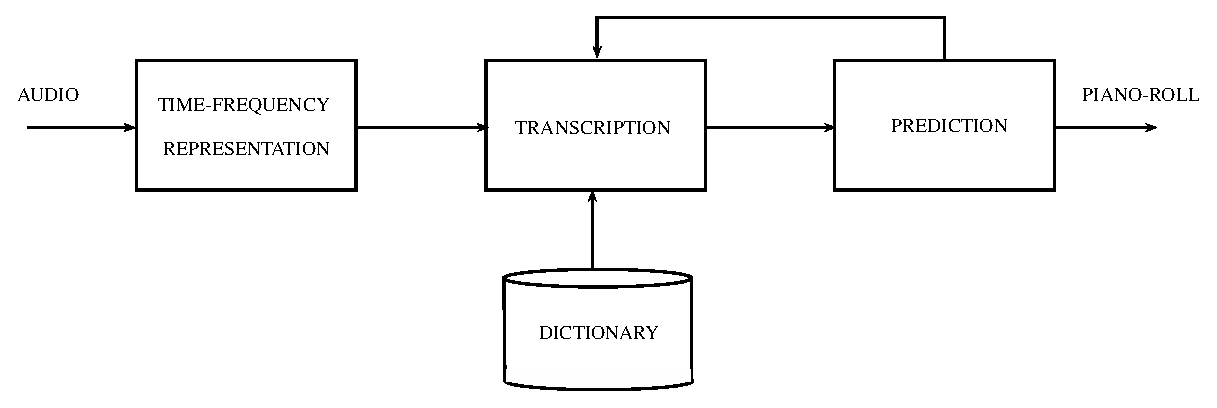
\includegraphics{figures/FigSystem.eps} 
 }
 \caption{Proposed system diagram.}
 \end{center}
 \label{fig:system}
\end{figure*}


\section{Evaluation} \label{sec:evaluation}

\subsection{Dataset}

For testing the transcription system, we employ the Bach10 dataset \cite{Duan2010}, which is a freely available multi-track collection of multiple-instrument polyphonic music, suitable for multi-pitch detection experiments. It consists of ten recordings of J.S. Bach chorales, performed by violin, clarinet, saxophone, and bassoon. Pitch ground truth for each instrument is also provided. Due to the tonal and homogenous content of the dataset, it is suitable for testing the incorporation of music language models in a transcription system. For training the transcription system, pre-extracted and pre-shifted spectral templates are extracted for the instruments present in the dataset, using isolated note samples from the RWC database \cite{Goto2003}. 

\subsection{Metrics}

For evaluating the performance of the proposed system for multi-pitch detection, we employ the precision, recall, and F-measure metrics, which are commonly used in transcription evaluations \cite{MIREX}:
\begin{equation}
 \mathit{Pre} = \frac{N_{\mathit{tp}}}{N_{\mathit{sys}}},\ \
\ \mathit{Rec} = \frac{N_{\mathit{tp}}}{N_{\mathit{ref}}},\
\ \ \mathit{F} = \frac{2\cdot\mathit{Rec}\cdot\mathit{Pre}}{\mathit{Rec}+\mathit{Pre}}
\label{eq:PRF}
\end{equation}
where $N_{\mathit{tp}}$ is the number of correctly detected pitches, $N_{\mathit{sys}}$ is the number of detected pitches, and $N_{\mathit{ref}}$ is the number of ground-truth pitches. As in the public evaluations on multi-pitch detection carried out through the MIREX framework \cite{MIREX}, a detected note is considered correct is if its pitch is the same as the ground truth pitch and its onset is within a 50ms tolerance interval of the ground-truth onset.

\subsection{Results}

Multi-pitch detection experiments are performed using the proposed system, with various configurations. A first configuration only considers the transcription system from Section \ref{sec:transcription}. A second configuration takes the output of the transcription system and gives it as input to the prediction system of Section \ref{sec:prediction}, where the final piano-roll is the output of the prediction step. A third configuration is the one presented in Section \ref{sec:combination}, where the recording is re-transcribed, having the prediction as a prior information for estimating the pitch activations. For the prediction system, experiments were made using both the RNN-NADE and the RNN.

Results using the various system configurations are displayed in Table \ref{tab:results}. As an example of the proposed system's performance, the transcription output using the 3rd configuration is displayed for a recording from the Bacg10 dataset in Fig. \ref{fig:Transcription}, along with the ground truth for the same recording.

For comparison with the method of \cite{Duan2010} (where the Bach10 dataset was first introduced), the proposed method using the frame-based accuracy metric which is defined in the same paper by Duan et al., reaches 74.3\% for the NADE-HF using the 3rd configuration, whereas the method of \cite{Duan2010} reaches 69.7\% (with unknown polyphony).

\begin{table}[t]
 \begin{center}
 \resizebox{230pt}{!}{
 \begin{tabular}{|l|c|c|c|}
  \hline
  \textbf{Configuration} & $\mathit{F}$ & $\mathit{Pre}$ & $\mathit{Rec}$  \\ \hline 
  Configuration 1 & 62.02\%  & 58.51\% & 66.12\% \\ \hline
  Configuration 2 - NADE & 62.62\% & 59.70\% & 65.92\% \\ \hline
  Configuration 3 - NADE & 64.08\% & 61.96\% & 66.44\% \\ \hline
  Configuration 2 - RNN & 62.29\% & 59.08\% & 65.98\% \\ \hline
  Configuration 3 - RNN & 63.85\% & 61.14\% & 66.90\% \\ \hline  
  Configuration 2 - NADE-HF & 62.20\% & 59.14\% & 65.68\% \\ \hline
  Configuration 3 - NADE-HF & \textbf{65.16}\% & \textbf{62.80}\% & \textbf{67.78}\% \\ \hline  
  Configuration 2 - RNN-HF & 62.44\% & 59.28\% & 66.07\% \\ \hline
  Configuration 3 - RNN-HF & 62.87\% & 60.03\% & 66.11\% \\ \hline    
 \end{tabular}
 }
\end{center}
 \caption{Transcription results using various system configurations.}
 \label{tab:results}
\end{table}

\begin{figure}
 \resizebox{230pt}{!}{
 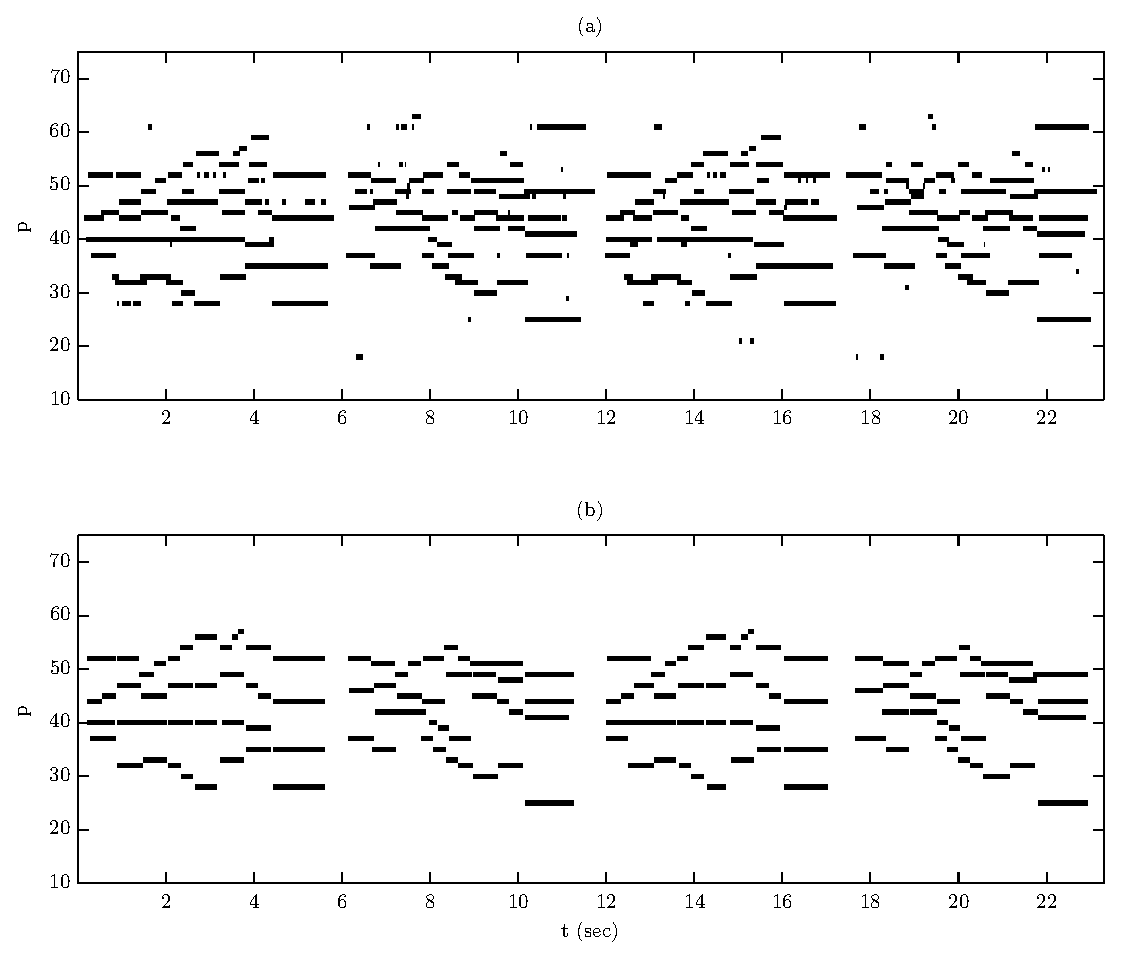
\includegraphics{figures/FigTranscription.eps}
 }
 \caption{Transcription example for recording  ``Ach Lieben Christen'' from the Bach10 dataset. (a) The output of the transcription-predicton system using the 3rd configuration, with the NADE-HF. (b) The pitch ground truth of the recording.}
 \label{fig:Transcription}
\end{figure}



\section{Conclusions} \label{sec:conclusions}

In this paper, we proposed a system for automatic music transcription which incorporated prior information from a polyphonic music prediction model based on recurrent neural networks. The acoustic transcription model was based on probabilistic latent component analysis, and information from the prediction system was incorporated using Dirichlet priors. Experimental results using the Bach10 dataset of multiple-instrument recordings showed that there is a significant improvement of 3\% in terms of F-measure, with statistical significance supported by \cite{BenetosThesis}, when combining a music language model with an acoustic transcription model instead of using an acoustic-only transcription system.

In the future, we would like to evaluate the proposed system using language models trained from different sources to see if this helps the MLMs generalize better. In addition, we aim to evaluate the proposed model on additional datasets of multiple-instrument polyphonic music. We will also investigate different system configurations, by bootstrapping the system for demonstrating that an improved transcription can lead to an improved prediction, and so on. We will also investigate the effect of using different RNN architectures like Long Short Term Memory (LSTM) and bi-directional RNNs and LSTMs. Finally, we would like to extend and improve the current models for high-dimensional sequences to better fit the requirements for music language modelling. 

% In the unusual situation where you want a paper to appear in the
% references without citing it in the main text, use \nocite
\nocite{langley00}

\bibliography{bibliography}
\bibliographystyle{icml2014}

\end{document} 


% This document was modified from the file originally made available by
% Pat Langley and Andrea Danyluk for ICML-2K. This version was
% created by Lise Getoor and Tobias Scheffer, it was slightly modified  
% from the 2010 version by Thorsten Joachims & Johannes Fuernkranz, 
% slightly modified from the 2009 version by Kiri Wagstaff and 
% Sam Roweis's 2008 version, which is slightly modified from 
% Prasad Tadepalli's 2007 version which is a lightly 
% changed version of the previous year's version by Andrew Moore, 
% which was in turn edited from those of Kristian Kersting and 
% Codrina Lauth. Alex Smola contributed to the algorithmic style files.  
